\documentclass[12pt]{article}

% This first part of the file is called the PREAMBLE. It includes
% customizations and command definitions. The preamble is everything
% between \documentclass and \begin{document}.

\usepackage[margin=1in]{geometry}  % set the margins to 1in on all sides
\usepackage{graphicx}              % to include figures
\usepackage{amsmath}               % great math stuff
\usepackage{amsfonts}              % for blackboard bold, etc
\usepackage{amsthm}                % better theorem environments
\usepackage{amssymb} 
\usepackage{mathptmx}
\usepackage{graphicx}
\usepackage{enumerate}
\usepackage{listings}
\usepackage{xcolor}
\usepackage{array}

% various theorems, numbered by section

\newtheorem{thm}{Theorem}[section]
\newtheorem{lem}[thm]{Lemma}
\newtheorem{prop}[thm]{Proposition}
\newtheorem{cor}[thm]{Corollary}
\newtheorem{conj}[thm]{Conjecture}
\newtheorem{mydef}[thm]{Definition}


\lstset{
	basicstyle          =   \sffamily,          
	keywordstyle        =   \bfseries,          
	commentstyle        =   \rmfamily\itshape,  
	stringstyle         =   \ttfamily,  
	flexiblecolumns,                
	numbers             =   left,   
	showspaces          =   false,  
	numberstyle         =   \fontsize{5}{skip},    
	showstringspaces    =   false,
	captionpos          =   t,      
	frame               =   lrtb,   
}

\lstdefinestyle{cpp}{
	language        =   cpp, 
	basicstyle      =   \fontsize{5}{skip},
	numberstyle     =   \fontsize{5}{skip},
	keywordstyle    =   \color{blue},
	keywordstyle    =   [2] \color{teal},
	stringstyle     =   \color{magenta},
	commentstyle    =   \color{red}\ttfamily,
	breaklines      =   true,   
	columns         =   fixed,  
	basewidth       =   0.5em,
}
\begin{document}


\title{ CSE 102 Spring 2021\\
	Advanced Homework Assignment 5}

\author{Jaden Liu \\ 
University of California at Santa Cruz\\
Santa Cruz, CA 95064 USA }

\maketitle


\section{AdvHW5} 

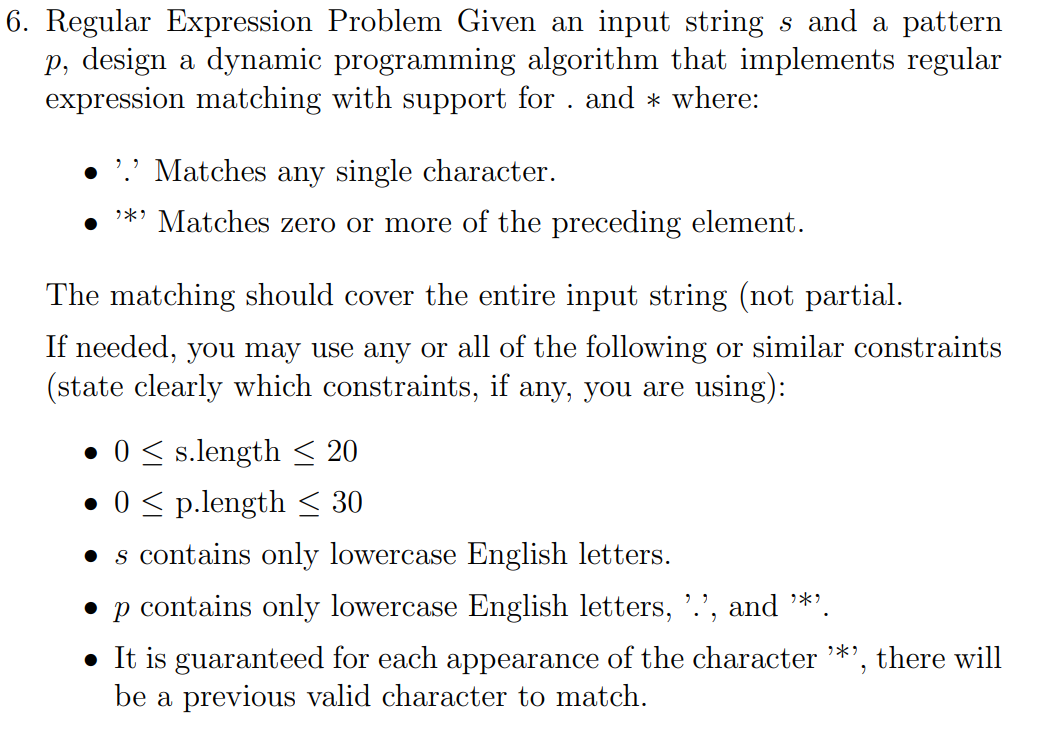
\includegraphics[scale=0.35]{adv_6.png}
\begin{proof}[Solution]
	We can come up with a 2-dimensional table c[i][j] to represent if first j arugments p[j] matches to first i elements s[i].\\
	1. Proof of optimality
	
	For this question, it satisfy the principle of optimality, which we can prove by contradiction. Let i = len(s), j = len(p), then we have an optimal solution for the question, let $0<k<i$ and c[k][j-2] or c[k][j-1], depending on if there is a "*", to be the optimal solution for previous matches of substring. Assume k is not the optimal match, then there exist l position in substring for optimal previous math. Then we can replace k with l to obtain a better matches, which generates a contradiction that c[i][j] is the optimal one. Thus we prove it has the optimal structure.\\
	2.Recurrence
	
	We have two situation in when we are matching two strings:
	
	a) If the jth character of p is a lowercase letter, then we must match the same lowercase letter in s, that is:\\
	\begin{equation*}
		c[i][j]=
		\begin{cases}
			c[i-1][j-1], s[i]=p[j]\\
			false, s[i]\ne p[j]
		\end{cases}
	\end{equation*}
	In other words, if the i-th character of s is not the same as the j-th character of p, the matching cannot be performed; Otherwise, we can match the last character of the two strings, and the complete matching result depends on the front part of the two strings.
	
	b)If the j-th character of p is "*", then we can match the j-th character of p any number of times.
	\begin{equation*}
		c[i][j]=
		\begin{cases}
			c[i-1][j-2], no\ match\\
			c[i-2][j-2], one\ match\\
			c[i-3][j-2], three\ matches\\
			\vdots\\
			c[i-1-k][j-2], k\ matches
		\end{cases}
	\end{equation*}
	Or, easily written as:\\
	\begin{equation*}
	c[i][j]=
	\begin{cases}
		c[i][j-2], no\ match\\
		c[i-1][j], one\ or\ multiple\ matches\\
	\end{cases}
	\end{equation*}
	It's because when we have a match, just repeat this	comparison it with previous character in s until reaching an difference.
	
	c) If j-th character is ".", then we must have a match.\\
	Then we have final recurrence:
	\begin{equation*}
	c[i][j]=
	\begin{cases}
		if\ j\ lower\ case:\begin{cases}
			c[i-1][j-1], s[i]=p[j]\\
			false, s[i]\ne p[j]
		\end{cases}\\
		if\ j\ equals\ "*":
		\begin{cases}
			c[i][j-2], no\ match\\
			c[i-1][j], one\ or\ multiple\ matches\ or\ j-1\ is\ "."\ \\
		\end{cases}\\
		if\ j\ equals\ ".":
		\begin{cases}
			c[i-1][j-1]
		\end{cases}		
	\end{cases}
	\end{equation*}\\

\begin{lstlisting}[language={python},numbers=left,numberstyle=\tiny,%frame=shadowbox,  
	rulesepcolor=\color{red!20!green!20!blue!20},  
	keywordstyle=\color{blue!70!black},  
	commentstyle=\color{blue!90!},  
	basicstyle=\ttfamily]  

	recurrence(c[][],i,j):
		if i=0 and j=0
			return true
		if j == "*":
			if s[i] != p[j]:
				c[i][j] = recurrence(c[][],i,j-2)
			else:
				c[i][j] = recurrence(c[][],i-1,j)
		elif j == ".":
			c[i][j] = recurrence(c[][],i-1,j-1)
		elif j == [a-z]:
			if s[i] == p[j]:
				c[i][j] = recurrence(c[][],i-1,j--1)
			else:
				return false
	return 
\end{lstlisting}
	3. DP algorithm 
	\begin{lstlisting}[language={python},numbers=left,numberstyle=\tiny,%frame=shadowbox,  
		rulesepcolor=\color{red!20!green!20!blue!20},  
		keywordstyle=\color{blue!70!black},  
		commentstyle=\color{blue!90!},  
		basicstyle=\ttfamily]  
		
	fill(len(s),len(p))
		c[][] = string [len(s)][len(p)]
		for i=0 to len(s):
			for j=0 to len(p): # fill the table 
					# from top to down, left to right
				if p[j] == "*":
					if match(i,j-1):
						c[i][j] = c[i][j-2]
					else:
						c[i][j] = c[i-1][j]
				elif p[j] == [a-z]:
					if match(i,j):
						c[i][j] = c[i-1][j-1]
					else:
						c[i][j] = false
				elif p[j] == ".":
					c[i][j] = c[i-1][j-1]
	return c[][]
	\end{lstlisting}
	4. Complexity
	
	Since we only have two loops that loop over m = len(s) and n = len(p) times, our time complexity is O(mn). Space complexity is O(mn) as well because we create a m*n matrix to save the result.\\
	5. Example 
	
	The first step is to initialize the first column to true to represent it will match for empty string.\\
	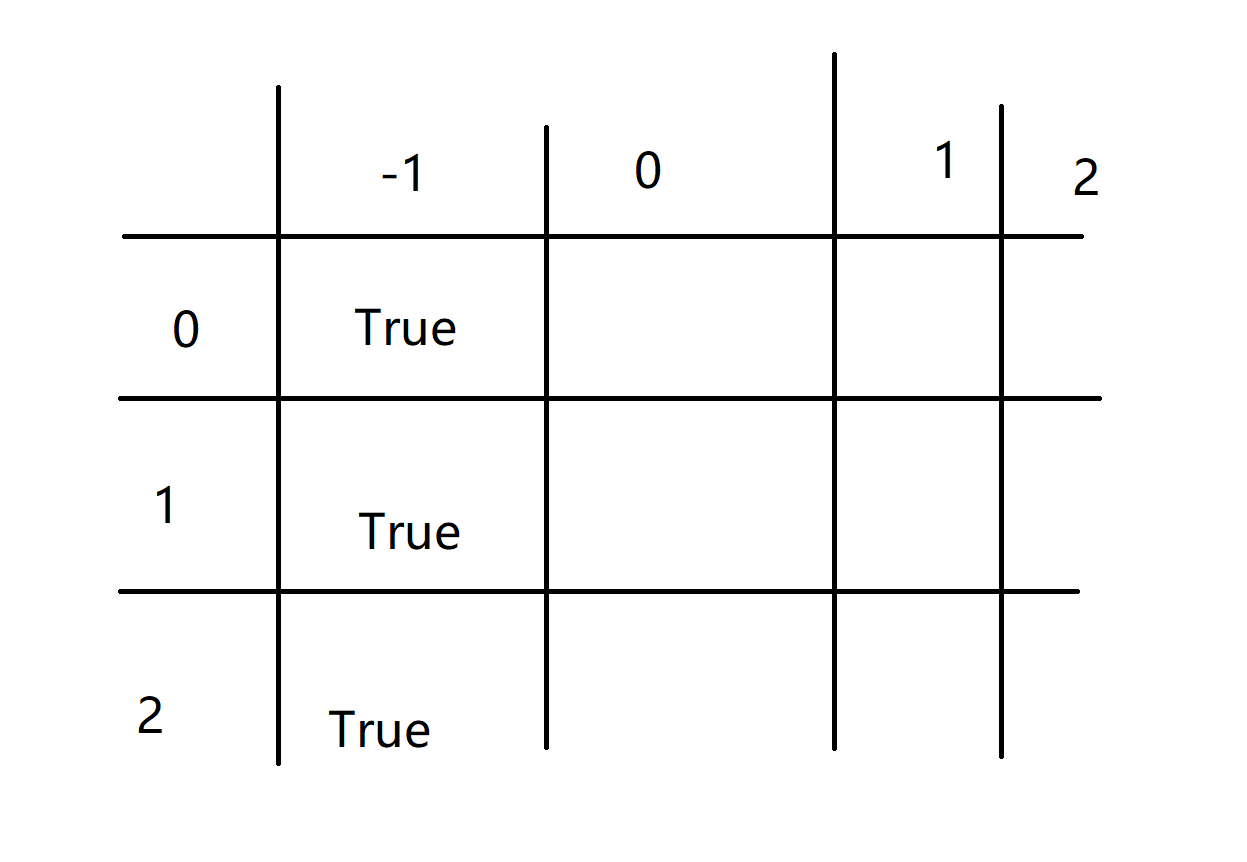
\includegraphics[scale=0.3]{s0.png}\\
	The first row is to check ("a","a"), ("a","a*"), ("a","a*b"), which is true, true, false\\
	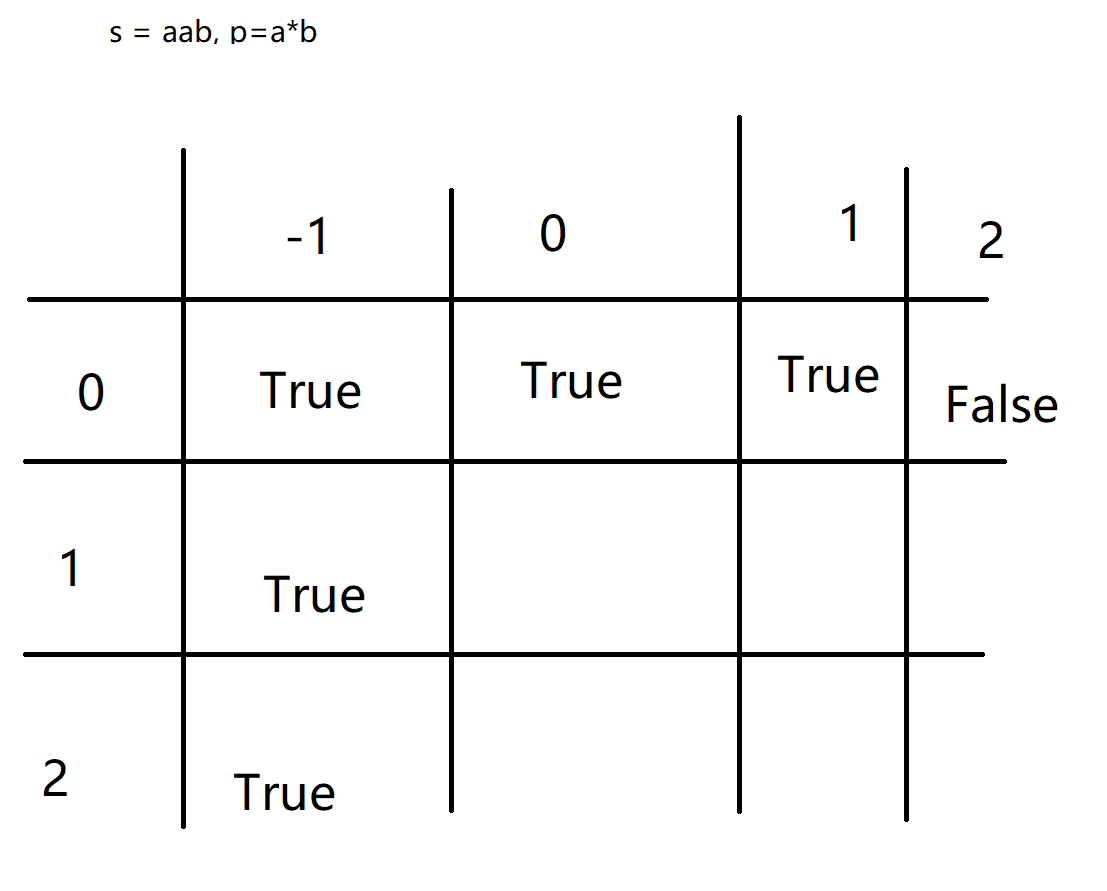
\includegraphics[scale=0.3]{s1.png}\\
	The second row is to check ("aa","a"), ("aa","a*"), ("aa","a*b"), which is false, true, false\\
	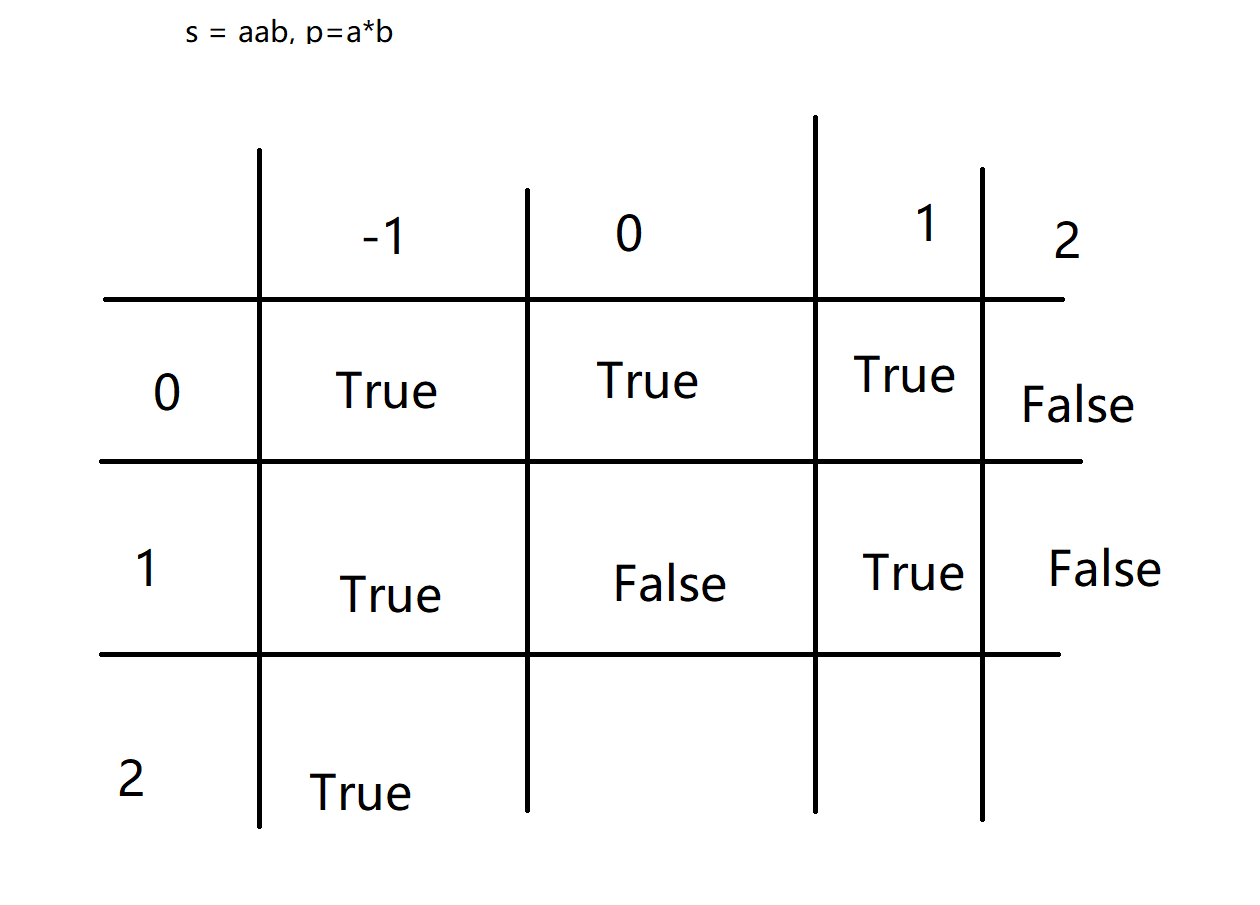
\includegraphics[scale=0.3]{s2.png}\\
	The third row is to check ("aab","a"), ("aab","a*"), ("aab","a*b"), which is false, false, true\\
	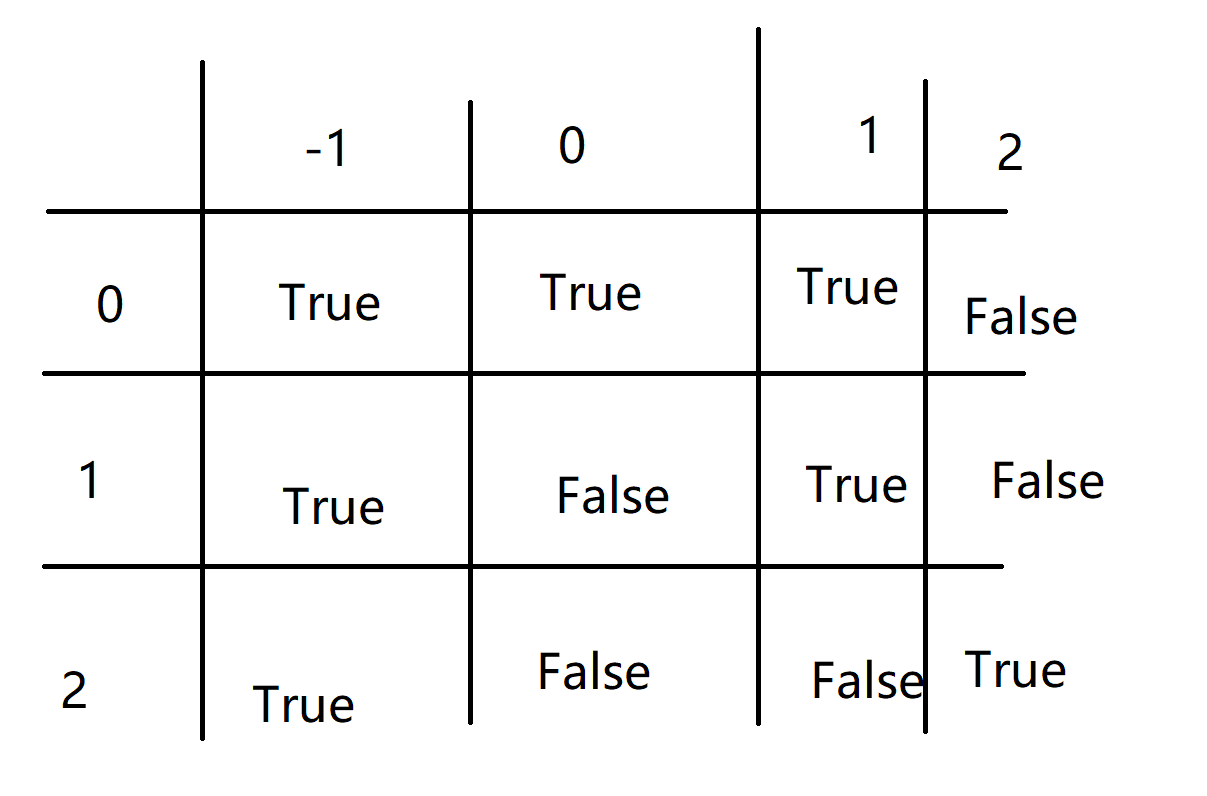
\includegraphics[scale=0.3]{s3.png}\\
\end{proof}


\end{document}
